%----------------------------------------------------------------------------------------
%	Capítulo 4
%----------------------------------------------------------------------------------------

\pagestyle{myportland}
\pagenumbering{arabic}
\doublespacing
\chapter[\quad\quad\quad\quad ----- Antecedentes]{\\ Antecedentes}
\thispagestyle{myportland}

%% NUEVA SECCIÓN X.X
\section{Descripción del sistema conceptual}
\label{sec:descripcion del sistema conceptual}

El presente trabajo es la continuación del trabajo \textit{Dise{\~{n}}o conceptual de clasificadora y contadora de truchas arco{\'{i}}ris (Oncorhynchus mykiss) de 10 a 20 cent{\'{i}}metros para la crianza de truchas en la Laguna de Paucarcocha}\footnote{\cite{DiazVergara2020}}. En la Figura \ref{fig:concepto optimo dibujo y virtual} se muestra el bosquejo del concepto de solución óptimo como su virtualización.

\begin{myfigure}[H]
	\centering
	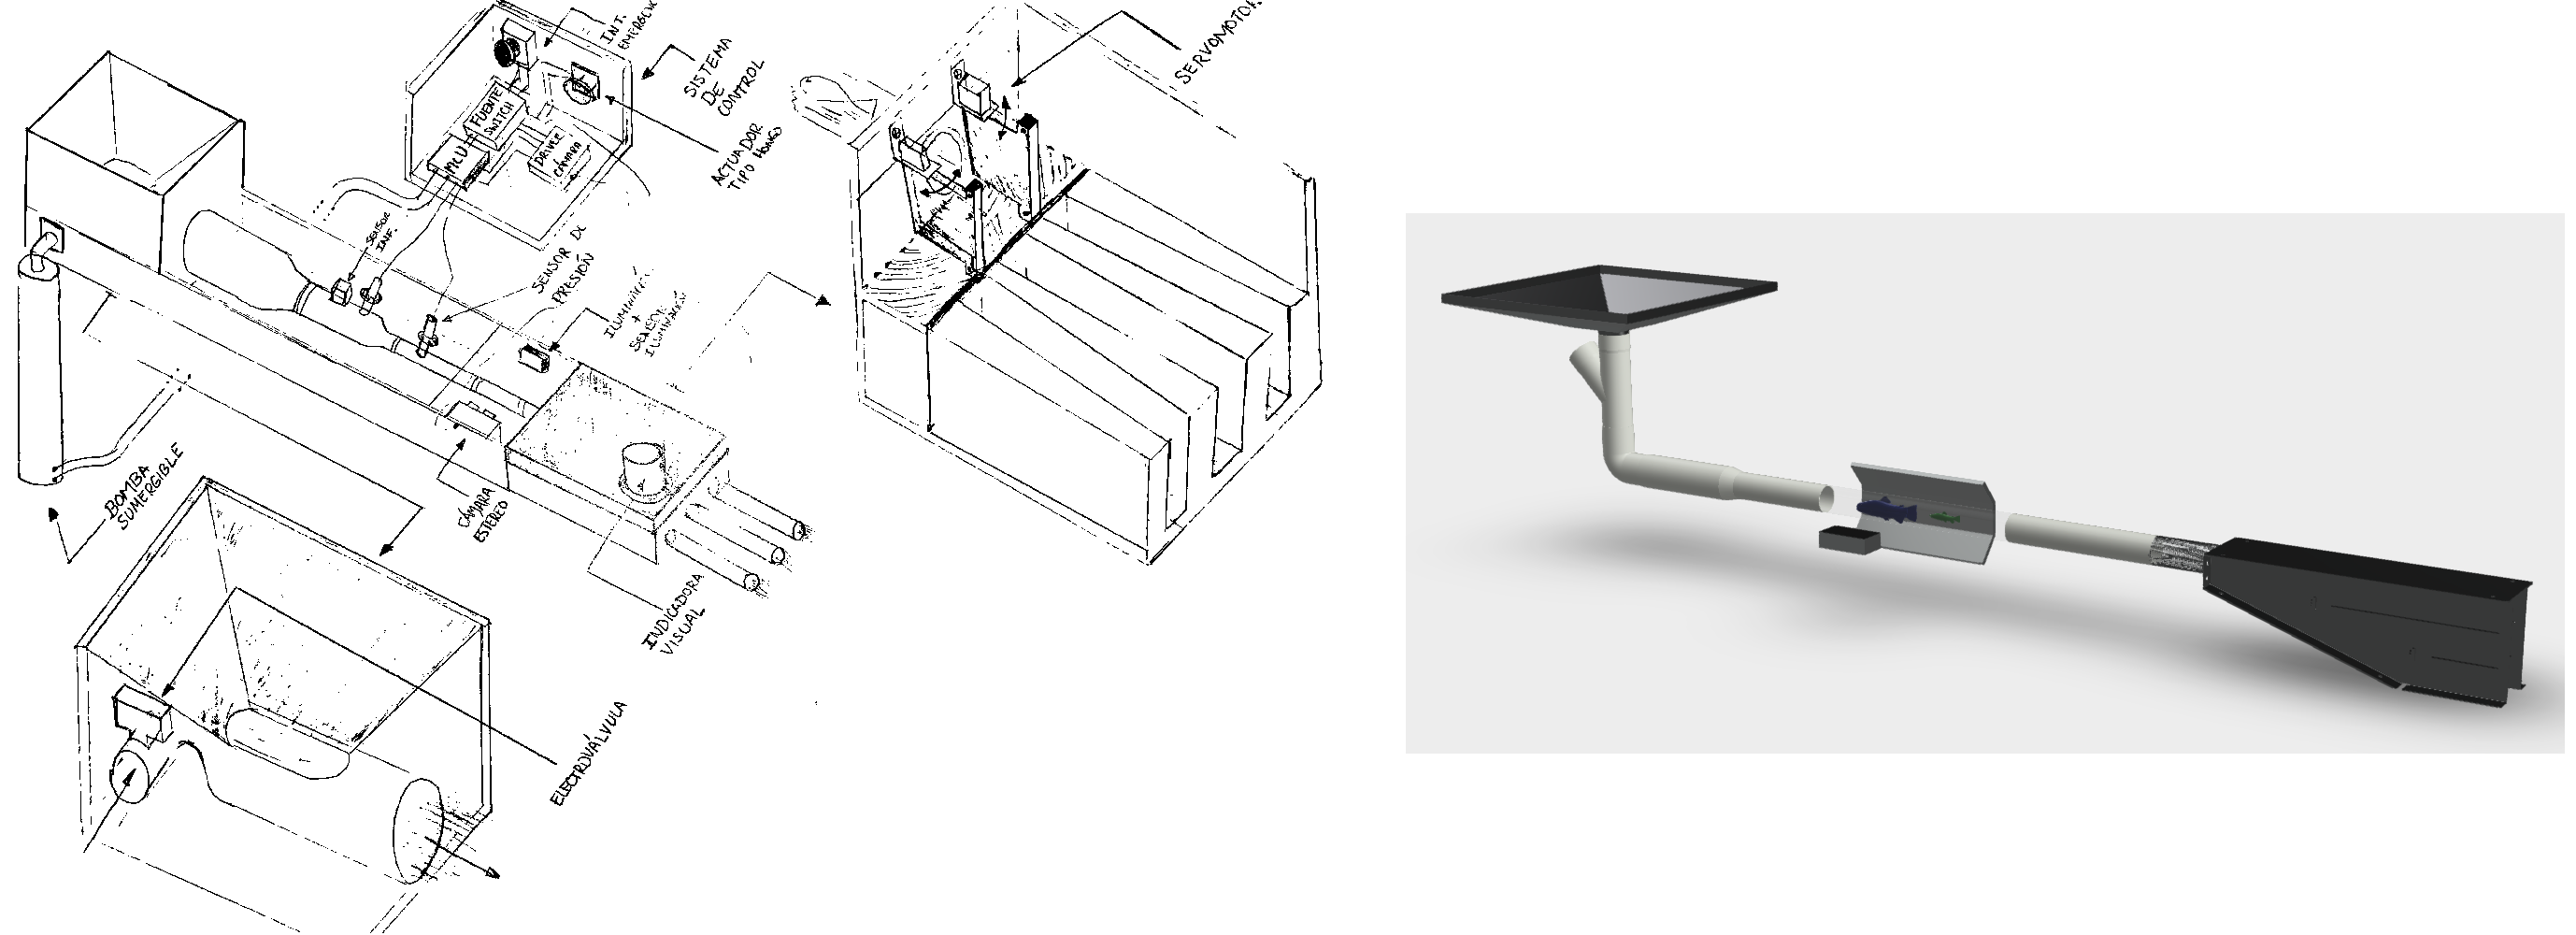
\includegraphics[width=1\textwidth]{chapter4/concepto optimo dibujo y virtual.png}
	\caption{Dibujo del concepto óptimo}
	\begin{myflushcenter}
		Fuente: \cite{DiazVergara2020}.
	\end{myflushcenter}
	\label{fig:concepto optimo dibujo y virtual}
\end{myfigure}

El desarrollo de ingeniería del concepto se realizó en el programa \textit{Fusion 360}\footnote{\textit{"Integrated CAD, CAM, CAE, and PCB software"}. \href{https://www.autodesk.com/products/fusion-360/overview}{Enlace}}. Tanto los diseños como renders\footnote{Imágenes procesadas de un diseño para ser foto-realistas.} pueden ser visualizados online en la web. En la Sección \ref{sec:desarrollo de diseno mecatronico integral} se explica a detalle el proceso de diseño y sus etapas.

%% NUEVO SUBSECCION X.X
\section{Objetivos}

Se presenta el objetivo general y los objetivos específicos del presente trabajo.

%% NUEVA SUB-SUB-SECCION X.X.X
\subsection{Objetivo general}

Realizar el diseño integral (de ingeniería) de una máquina clasificadora y contadora de truchas arcoíris (CCT) de 15 a 20 centímetros a partir del diseño conceptual previo\footnote{\cite{DiazVergara2020}}.

%% NUEVA SUB-SUB-SECCION X.X.X
\subsection{Objetivos específicos}

\begin{itemize}
	\item Recolectar imágenes para formar una base de datos para el algoritmo de detección de truchas. 
	%%%%%%%%%%%%%%%%%%%%%%%%%%%%%%%%%%%%%%%%%%%%%%%%%%%%%%%%%%%%%%%%%%%%%%%%%%%%%%%%%%%%%%%
	%\textcolor{blue}{[BORRADOR] ¿Alcanzará el tiempo o uso una red neuronal pre-entrenada? [/BORRADOR]} 
	%%%%%%%%%%%%%%%%%%%%%%%%%%%%%%%%%%%%%%%%%%%%%%%%%%%%%%%%%%%%%%%%%%%%%%%%%%%%%%%%%%%%%%%
	\item Desarrollar el procesamiento de imágenes para la detección y conteo de truchas arcoíris.
	%\item Orientar el desarrollo del proyecto hacia una máquina de bajo costo y con durabilidad.
	\item Realizar pruebas de los algoritmos, análisis de falla mecánica y presentar resultados de los algoritmos de detección, conteo y control del sistema.
	\item Presentar una estimación de costos y comparar dicho monto con el estado del arte\footnote{\cite{DiazVergara2020}}.	
\end{itemize}


%% NUEVA SECCIÓN X.X
\section{Alcance}

El presente estudio abarca el diseño integral de la CCT que resulta en una máquina de menor costo para disminuir la mortalidad en el proceso de clasificación y conteo de truchas en lagos o lagunas. Asimismo, unifica tecnologías de la última generación para automatizar el proceso mencionado. Además, pretende ser la base de un desarrollo mecatrónico en la industria truchicola, la cual tiene un potencial no explotado en el Perú.











